\chapter{Results and Discussion}
\label{chap:discussion}
 In this chapter, several aspects of the project thesis will be discussed. The topic of fatigue of dynamic power cables applied offshore wind farms will be discussed based on the literature review and theory section, and whether this topic should be investigated further in the master thesis or not. The global and local model will be discussed in modeling in SIMA RIFLEX and BFLEX and the results from testing of the model to see if they perform satisfactorily and are ready to be used in the master thesis. In addition, general simplifications and simplifications related to the models will be discussed. 
 \section{General Discussion of Topic and Case Study}
 Wind has been used by mankind for thousands of years. At first, it was used for propulsion of boats, later for grinding of cereal, and in the last century the wind turbine has emerged, converting the kinetic energy in wind flow to electrical energy. The last years this technology has become more efficient both in cost and in power, also bigger in size and capacity. As locations suitable for wind turbines on land are scarce, one of the newest advances for this industry has been moving the technology to the ocean. First with bottom fixed structures in shallow waters, but also several floating concepts have been proposed, allowing for wind far from shore in deep waters. Moving the wind turbine installations offshore demands high performance from the dynamic power cable, and this is one of the factors slowing down development of offshore wind.\\\\ Floating offshore wind farms are often placed on locations with rough weather conditions, and damage due to fatigue are highly relevant. From the long experience with oil and gas, dynamic flexible risers and their lifetime have been investigated for decades. The motions of a floating wind turbine will be very different from a semi-submersible platform, and there is not a lot of knowledge on the lifetime of dynamic power cables applied in offshore wind. It is therefore clear that gaining more knowledge about the lifetime of dynamic power cables applied in offshore wind farm is a very interesting topic, and definitely worth investigating further in the master thesis. \\\\ When it comes to choice of a case study, the OO-Star from Dr. Techn. Olav Olsen was chosen due to the previous familiarity with the project for the author, through a summer internship. OO-Star is part of a research project called Lifes50+ where different floating wind turbine designs and locations will be investigated. OO-Star it not fully developed, and has not yet been constructed. An advantage of choosing this concept is that there is a lot of information available on the website of Lifes50+. Another option could have been to use the Hywind concept that is already installed at the Hywind Scotland project, or one of the other concepts in the Lifes50+ project. The location of the case study was chosen to be West of Barra. This is the location in the project with the deepest water and with the most challenging weather conditions. It was thought that these factors would make the investigation of the lifetime of the power cable the most interesting in terms of fatigue. As the design is very interesting and the information about the design and the met-ocean data are more available than for other alternatives, this has proved to be an exciting case, and OO-Star will continue to be used for the master thesis next semester. 
\section{Discussion of Modeling Methodology}
\subsection{Global Model}
 The global model was modeled in SIMA RIFLEX. The model consists of the total cable configuration and is attached to a point a calculated distance from the center of gravity of the OO-Star. The point will have its motions in accordance with the support structure of the OO-Stare due to the transfer functions provided by Dr. Techn. Olav Olsen. The configuration is the characteristic lazy wave, which is simple to model, but hard to ensure that the touchdown is stable. Usually, this configuration has a thether on the bottom to keep the touchdown stable. As this can be difficult to model in SIMA RIFLEX, and the area of interest is the vessel hang off, this was not included in the global model. The main design criteria for the configuration of the global model was that the max curvature could not be exceeded anywhere in the cable. The configuration was determined through testing and failing, and this process could have been done in a more systematic way, and the cable configuration could probably be optimized. \\\\ The wind conditions have been simplified significantly for the global model. The only way the wind is taken into consideration is with the three different positions, near, neutral and far, with the near position being max wind from the east and far position is max wind from the west. The far position was calculated as 20\% of the water depth and it is assumed that the system is linear. Because of this, the fatigue damage on the power cable will mainly be from the waves at the chosen location. The scatter diagram for the wind conditions at West of Barra is available and could be used to simulate the wind conditions at the location more realistically, however, this would make the model and the analyses more complex. Current is not included in the model, and this is another simplification.\\\\ To keep away from the sea states with resonance, the original scatter diagram for waves at West of Barra was adjusted somewhat. This only affects the most severe sea states that are very rare, and thus should not alter the fatigue damage very much.\\\\ The global model is significantly simplified compared to the realistic case, but it is believed that it is a good start to investigate the lifetime of a dynamic power cable applied in offshore wind, and the model could be developed further to become more complex and realistic later if needed. 
 
\subsection{Local Model}
The local model was created in BFLEX and was modeled from the inner layer and outwards. The dimensions of the different components in the cable are based on the dimensions of the three 95mm$^2$ conductors and guidance from Professor Svein Sævik. Another approach that could have been used was to select a specific cable cross section from a cable manufacturer and base the dimensions off its cross section. However, the majority of dynamic power cables are designed specifically for its use, and standardized models are rare. Only the very upper part of the cable is modeled as this is considered to be the area with the most damage. The friction models used to describe the contact between the layers could have been explored more and other alternative friction models could have been considered. \\\\ In real life, a conductor with area 95mm$^2$ consists of 19 wires. These are not modeled, and instead, equations developed by \cite{savik2014} will be used to determine the stress variation in the individual wires. Friction between the individual wires will thus not be included in the models, even though local friction between the layers have been proven to be of significance. The armouring layers are only modeled with 4 wires in each layer, but this is accounted for by scaling factor. \\\\ The contact element used to describe the contact between the conductors is HCONT454. This is a brand new element developed by Professor Svein Sævik and has actually not been used much in modeling before. Whether using this element will improve the modeling of the contact between the conductors or not is still unknown at this point. \\\\The dimensions of the bend stiffener are based on very rough calculations and guidance from Professor Svein Sævik. It has been commented on that it seems somewhat short, and this should be investigated further in the master thesis by making more thorough calculations. \\\\ The S-N curve to be used in the master thesis is found from the article by \cite{savik2014}. Other alternatives could have been investigated. 

\section{Results}
The desired results in this project thesis are confirmation that the two models are working and are ready to be used in the master thesis.
\subsection{Global Model}
To make sure the global model is working in a satisfactorily way, it was tested with the most severe sea state. The variables used in this test can be seen in table \ref{table:testglob}. The results from the test will be discussed in this section. \newline \newline
The static configuration for the three different wind conditions: 
\begin{figure}[H]
\subfloat[Near position\label{fig:cavS200}]
  {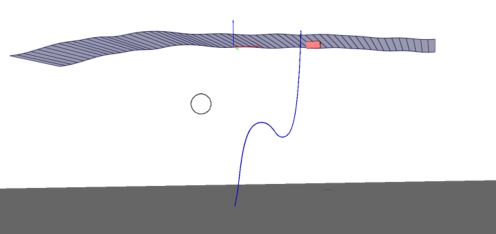
\includegraphics[width=.3\linewidth]{figures/staposnear}}\hfill
\subfloat[Neutral position \label{fig:cavS2500}]
  {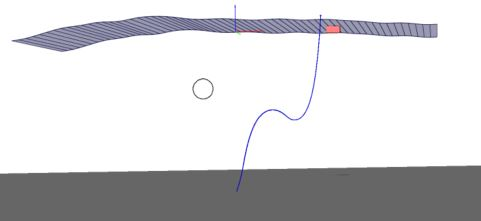
\includegraphics[width=.3\linewidth]{figures/statposneu}}\hfill
  \subfloat[Far position \label{fig:cavS5000}]
  {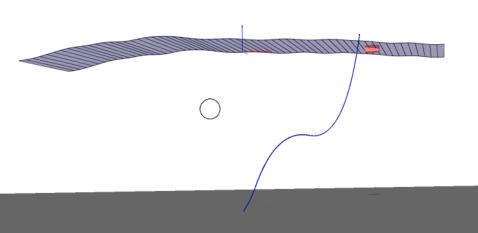
\includegraphics[width=.3\linewidth]{figures/statposfar}}\hfill
\caption[$\; \:$Static configuration for the global model]{Static configuration for the global model for different wind conditions}
\label{fig:statcon}
\end{figure}

\noindent Figure \ref{fig:statcon} shows the static configuration of the cable for the three different positions. It can be seen that the characteristic lazy wave shape is maintained both in the near position and the far position. \newline
\newline
The static configurations in the three different positions:
\begin{figure}[H]
\centering
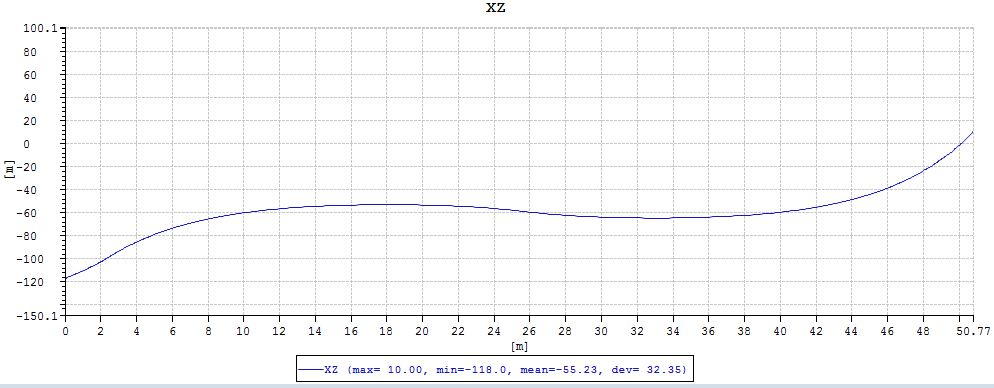
\includegraphics[scale=0.5]{figures/confignear}
\caption[$\; \:$Configuration for near position]{Configuration for near position}
 \label{fig:confignear}
\end{figure}

\begin{figure}[H]
\centering
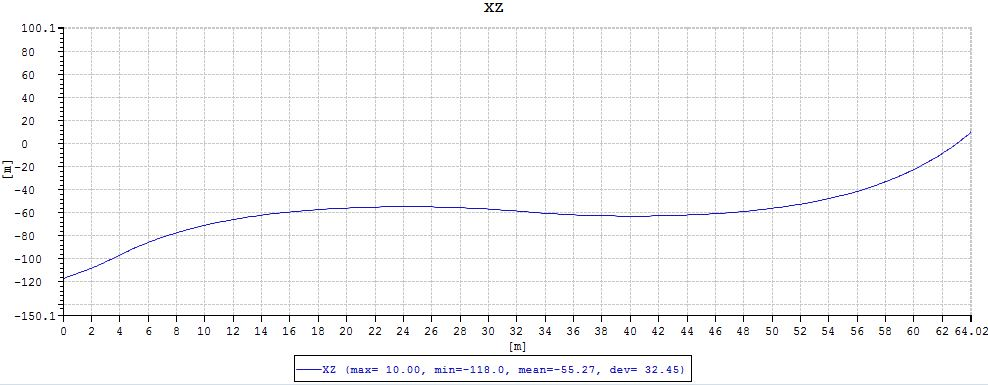
\includegraphics[scale=0.5]{figures/configneu}
\caption[$\; \:$Configuration for neutral position]{Configuration for neutral position}
 \label{fig:configneu}
\end{figure}

\begin{figure}[H]
\centering
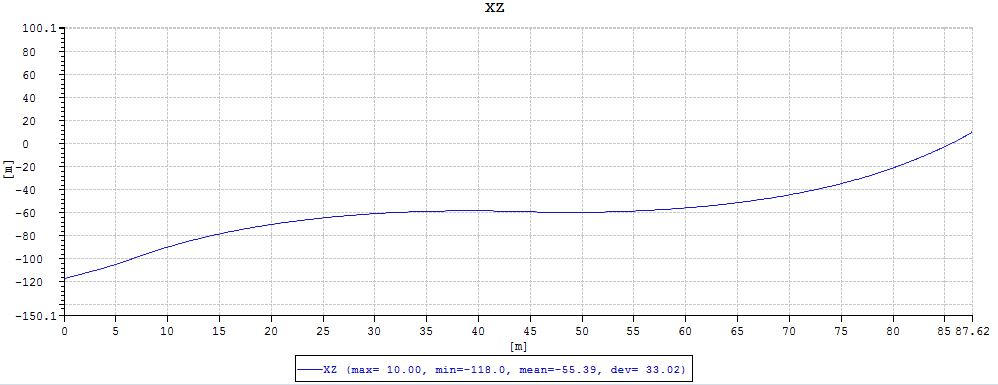
\includegraphics[scale=0.5]{figures/configfar}
\caption[$\; \:$Configuration for far position]{Configuration for far position}
 \label{fig:configfar}
\end{figure}
\noindent Figures \ref{fig:confignear}, \ref{fig:configneu} and \ref{fig:configfar} also show the static configurations for the different positions. The highest point of the curved buoyancy section is at its highest about 50m depth in the near position. Collision is therefore not very likely. \newline
\newline
\noindent The envelope curves for the curvatures:

\begin{figure}[H]
\centering
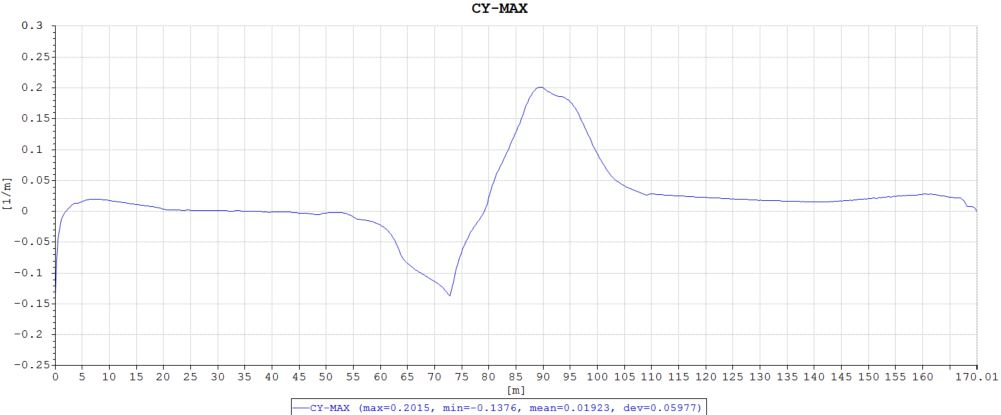
\includegraphics[scale=0.8]{figures/envcurvenear}
\caption[$\; \:$Curvature envelope for near position]{Curvature envelope for near position}
 \label{fig:envcurvenear}
\end{figure}

\begin{figure}[H]
\centering
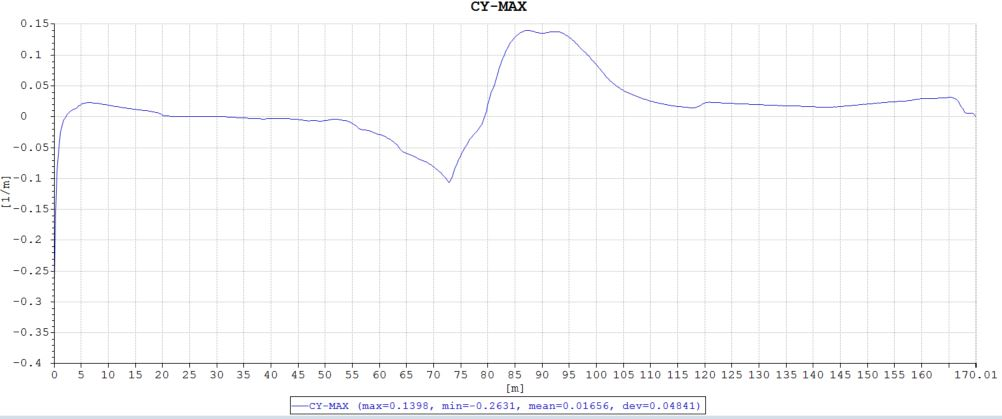
\includegraphics[scale=0.8]{figures/envcurveneu}
\caption[$\; \:$Curvature envelope for neutral position]{Curvature envelope for neutral position}
 \label{fig:envcurveneu}
\end{figure}

\begin{figure}[H]
\centering
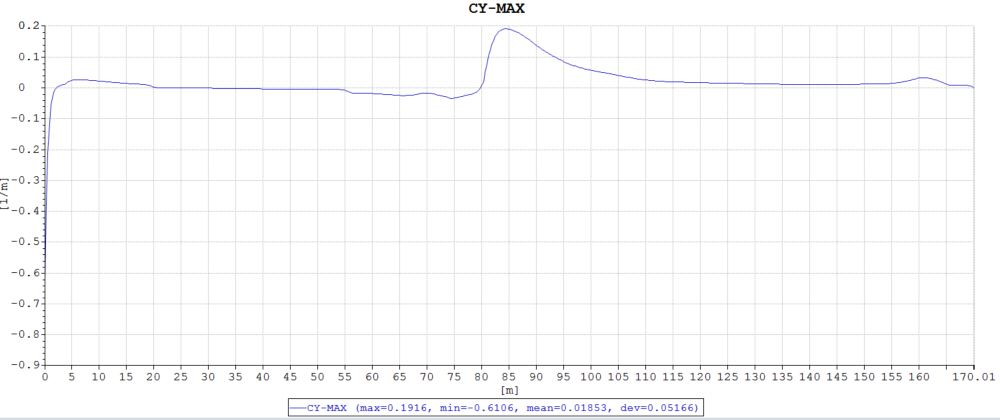
\includegraphics[scale=0.8]{figures/envcurvefar}
\caption[$\; \:$Curvature envelope for far position]{Curvature envelope for far position}
 \label{fig:envcurvefar}
\end{figure}
\noindent Figures \ref{fig:envcurvenear}, \ref{fig:envcurveneu} and \ref{fig:envcurvefar} show the envelope curve for the curvature over the length of the cable. It can be seen that the highest curvature occurs at -0.6106 $\frac{1}{m}$ at the anchoring in far position. This is only 44.65\% of the maximum allowed critical curvature of 1.3675$\frac{1}{m}$, giving a safety factor of 2.24. \newline
  \newline
 \noindent The max tension over the length of the cable

\begin{figure}[H]
\centering
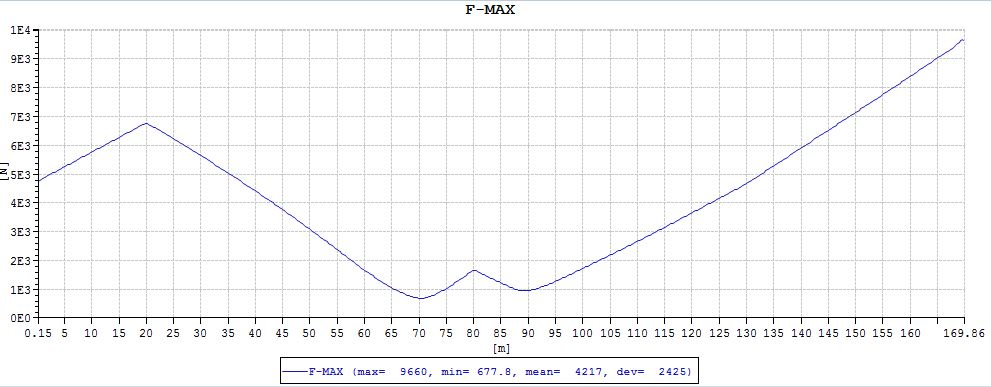
\includegraphics[scale=0.5]{figures/fmaxnear}
\caption[$\; \:$The max tension in near position]{The max tension over the length of the cable in near position}
 \label{fig:fmaxnear}
\end{figure}


\begin{figure}[H]
\centering
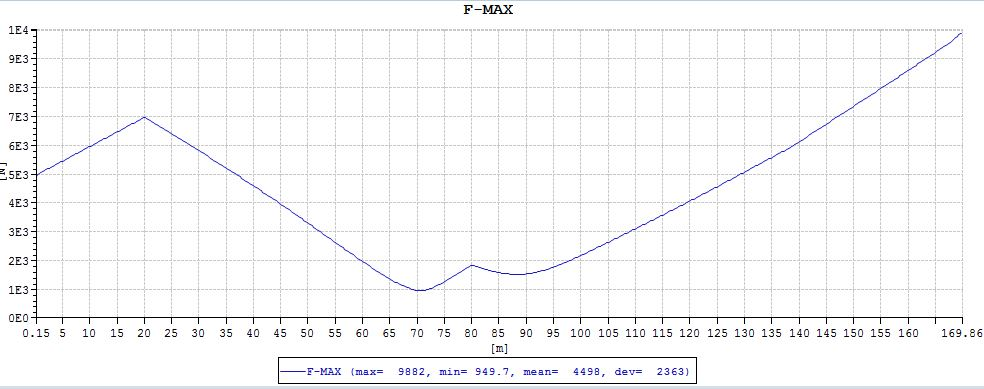
\includegraphics[scale=0.5]{figures/fmaxneu}
\caption[$\; \:$The max tension in neutral position]{The max tension over the length of the cable in neutral position}
 \label{fig:fmaxneu}
\end{figure}


\begin{figure}[H]
\centering
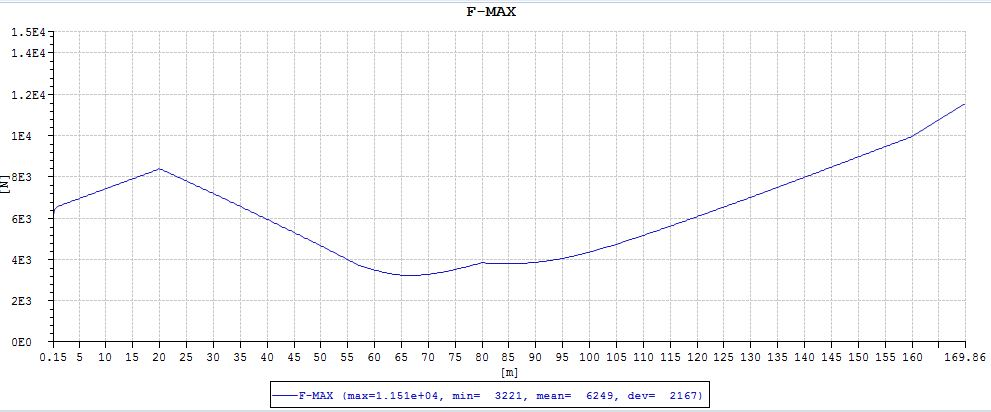
\includegraphics[scale=0.5]{figures/fmaxfar}
\caption[$\; \:$The max tension in far position]{The max tension over the length of the cable in far position}
 \label{fig:fmaxfar}
\end{figure}
\noindent Figures \ref{fig:fmaxnear}, \ref{fig:fmaxneu} and \ref{fig:fmaxfar} show the envelope curve for the max tension on the cable. From these figures it can be seen that the maximum tension occur at the very top of the cable as expected.\newline
 \newline 
 \noindent The minimum tension over the length of the cable
 
 \begin{figure}[H]
\centering
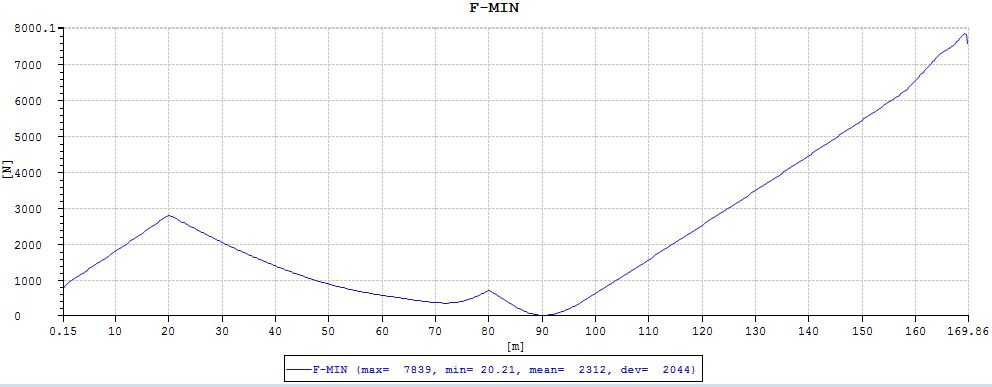
\includegraphics[scale=0.5]{figures/fminnear}
\caption[$\; \:$The minimum tension in near position ]{The minimum tension over the length of the cable in near position}
 \label{fig:fminnear}
\end{figure}


\begin{figure}[H]
\centering
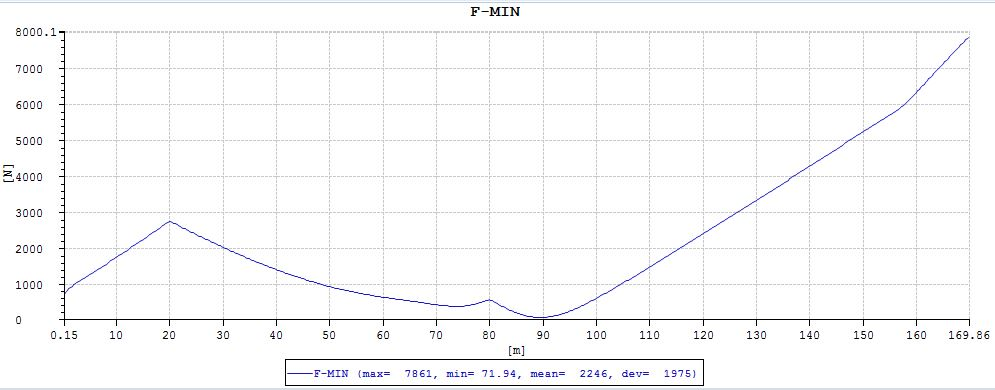
\includegraphics[scale=0.5]{figures/fminneu}
\caption[$\; \:$The minimum tension in neutral position ]{The minimum tension over the length of the cable in neutral position}
 \label{fig:fminneu}
\end{figure}


\begin{figure}[H]
\centering
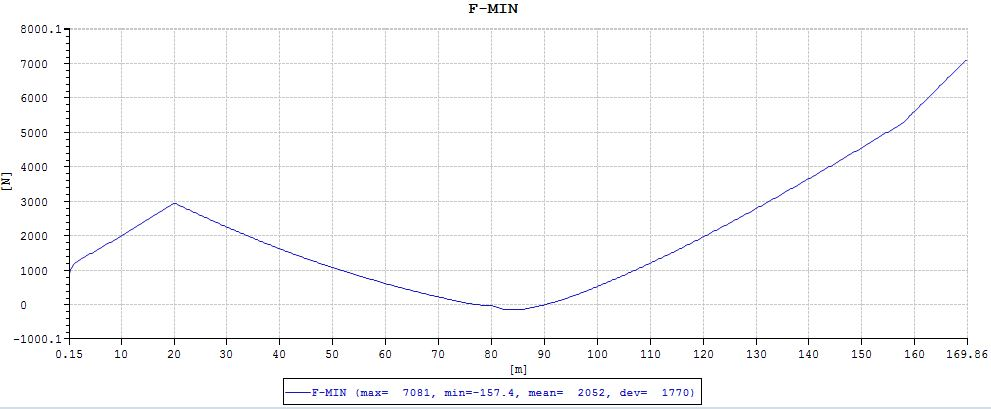
\includegraphics[scale=0.5]{figures/fminfar}
\caption[$\; \:$The minimum tension in far position ]{The minimum tension over the length of the cable in far position}
 \label{fig:fminfar}
\end{figure}
\noindent Figures \ref{fig:fminnear}, \ref{fig:fminneu} and \ref{fig:fminfar} show the envelope curve for the minimum force in the cable. From this it is concluded that there is no undesired compression at the anchoring of the cable in any of the positions.  
 \newline
 \newline
 \noindent The results discussed above confirms that the global model satisfies the key requirements so far, and that it will continue to be used in the master thesis. 

\subsection{Local Model}
The following figures show the local model and some of the layers: 

\begin{figure}[H]
\subfloat[Local model from the side with bend stiffener \label{fig:lm_total}]
  {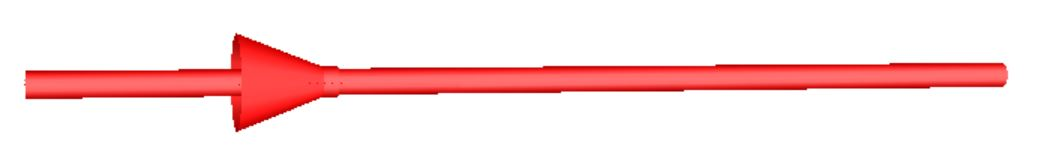
\includegraphics[width=.45\linewidth]{figures/lm_total}}\hfill
\subfloat[Cable cross section in local model \label{fig:lm_cross}]
  {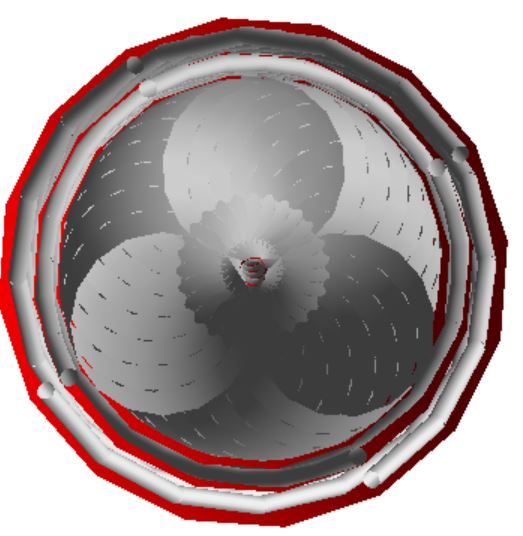
\includegraphics[width=.25\linewidth]{figures/lm_cross}}\hfill
\caption[$\; \:$Local model ]{Local model}
\label{fig:loc1}
\end{figure}
\noindent 

\begin{figure}[H]
\subfloat[Conductors \label{fig:single}]
  {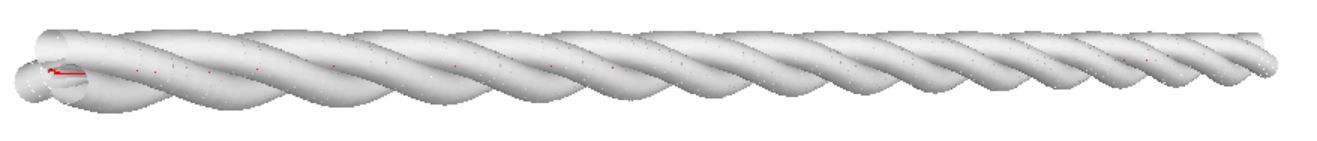
\includegraphics[width=.45\linewidth]{figures/lm_conductors}}\hfill
\subfloat[Armouring \label{fig:3phase}]
  {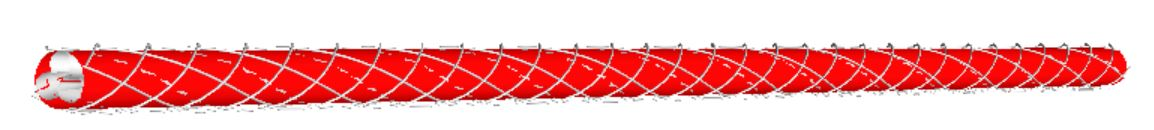
\includegraphics[width=.45\linewidth]{figures/lm_arm}}\hfill
\caption[$\; \:$Helical components in the local model ]{Helical components in the local model}
\label{fig:loc2}
\end{figure}

\noindent The local model was, as the global model, tested to see it it performs the way it should. The applied loads are presented in section \ref{sec:localtest}. The results from the test are presented in the plots below: 

\begin{figure}[H]
\centering
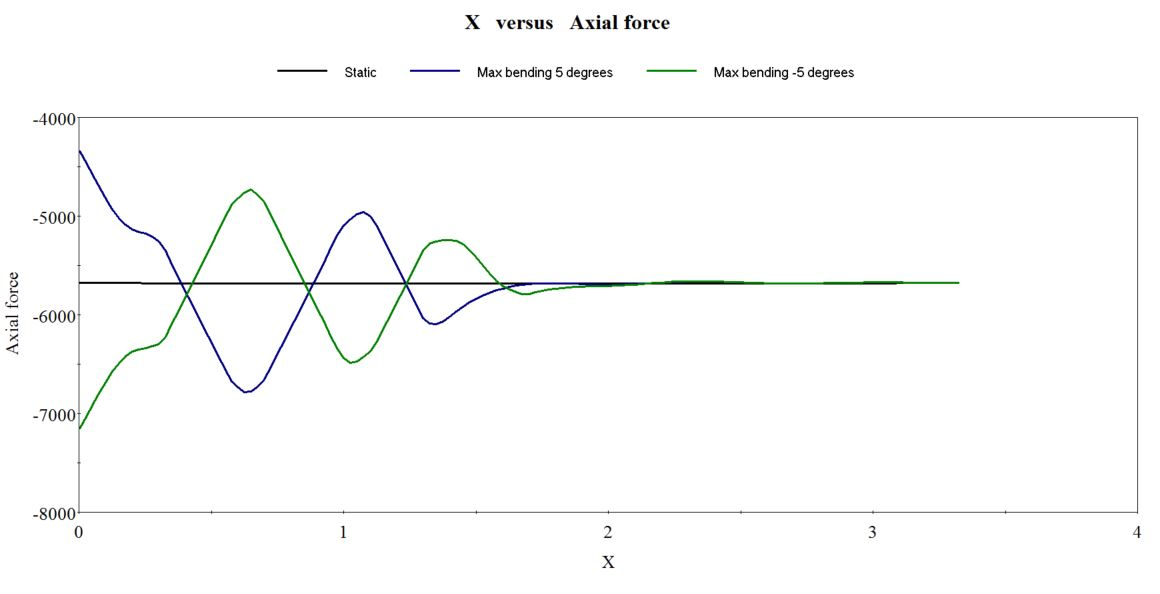
\includegraphics[scale=0.75]{figures/bflexax}
\caption[$\; \:$Axial force in conductors]{Axial force in conductors over length of cable [N]}
 \label{fig:bflexax}
\end{figure}
\noindent Figure \ref{fig:bflexax} shows the axial force distribution over the cable. With no bending, the axial force is about 6300N throughout the conductor. When bending is applied the axial force will have cyclic behavior due to friction.
\begin{figure}[H]
\centering
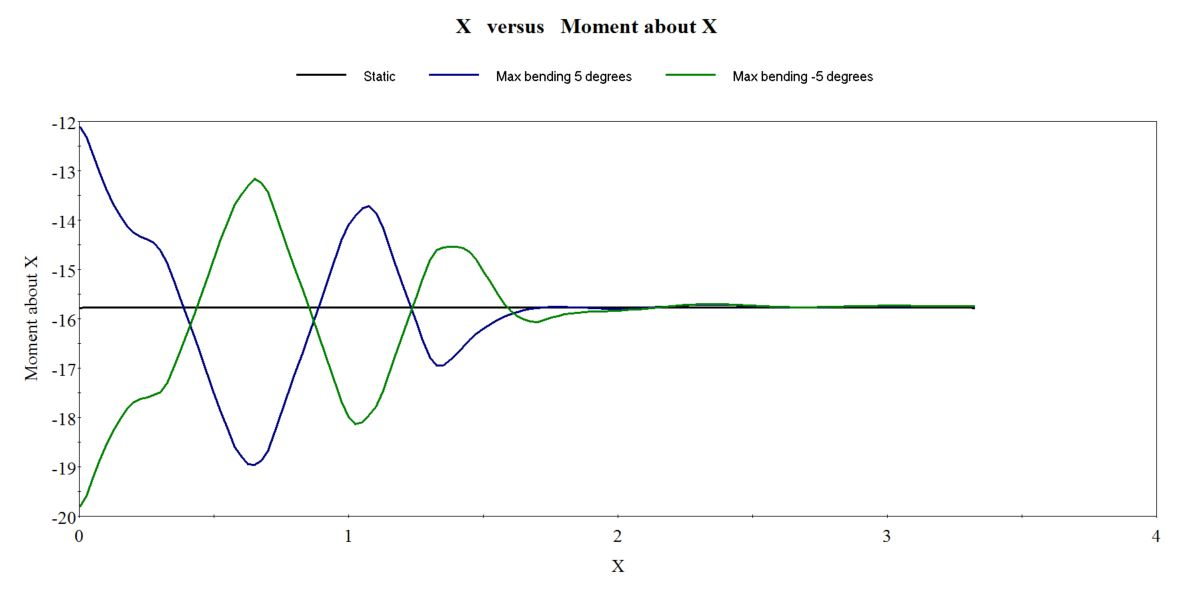
\includegraphics[scale=0.75]{figures/bflexmx}
\caption[$\; \:$Moment about X-Axis in conductors]{Moment about X-Axis in conductors over length of cable}
 \label{fig:bflexmx}
\end{figure}

\noindent Figure \ref{fig:bflexmx} shows the moment about the x-axis over the length of cable. The same tendency as in figure \ref{fig:bflexax} can be seen with a constant moment when there is no bending and cyclic moment when bending is applied. The plot for bending at 5 degrees is opposite of the plot for bending at -5 degrees as expected.  

\begin{figure}[H]
\centering
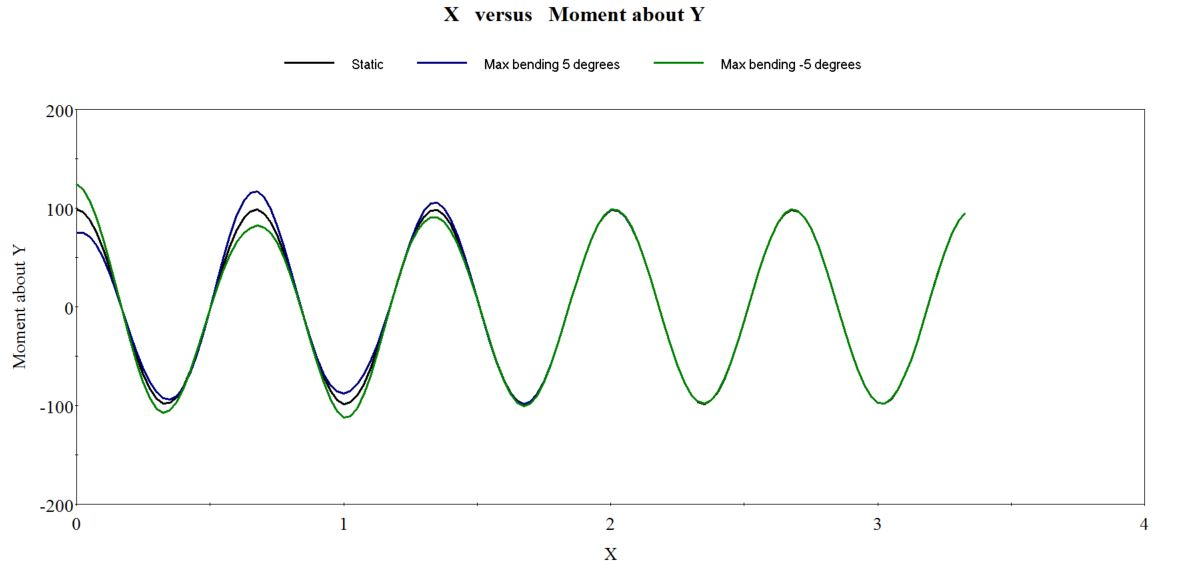
\includegraphics[scale=0.75]{figures/bflexmy}
\caption[$\; \:$Moment about Y-Axis in conductors]{Moment about Y-Axis in conductors over length of cable}
 \label{fig:bflexmy}
\end{figure}
\noindent Figure \ref{fig:bflexmx} displays the moment about the y-axis over the length of cable. The plot is cyclic as the conductor is helical. 

\begin{figure}[H]
\centering
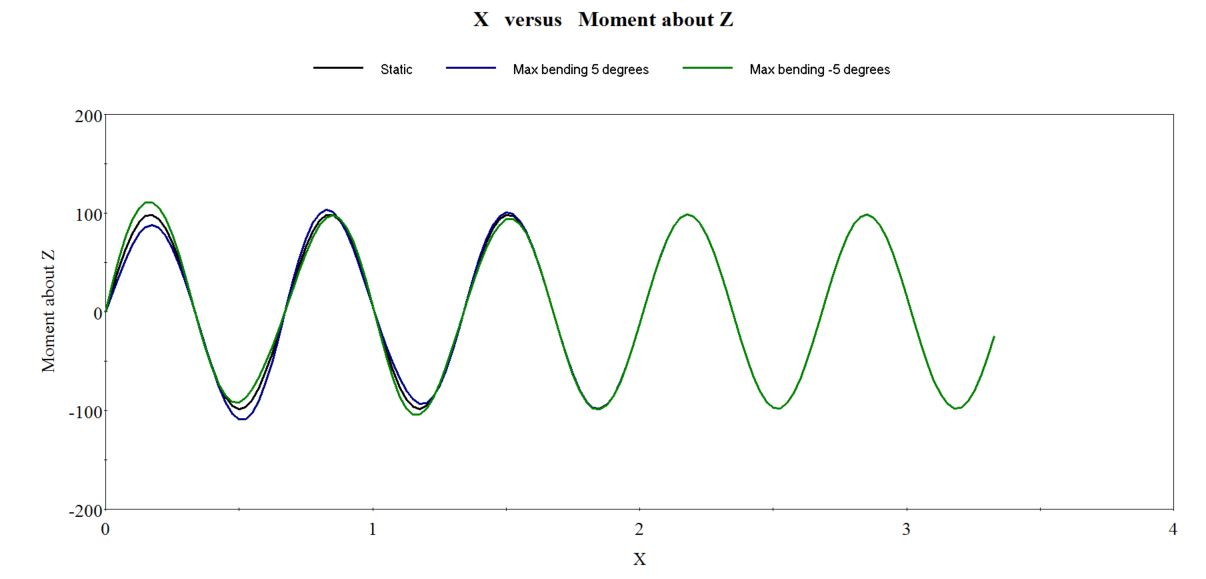
\includegraphics[scale=0.75]{figures/bflexmz}
\caption[$\; \:$Axial force in conductors]{Axial force in conductors over length of cable}
 \label{fig:bflexmz}
\end{figure}
\noindent Figure \ref{fig:bflexmx} displays the moment about the z-axis over the length of cable. The plot is cyclic for the same reason as the figure above. It can be observed that the moment about the Y-axis and the Z-axis are in opposite phase.  

\begin{figure}[H]
\centering
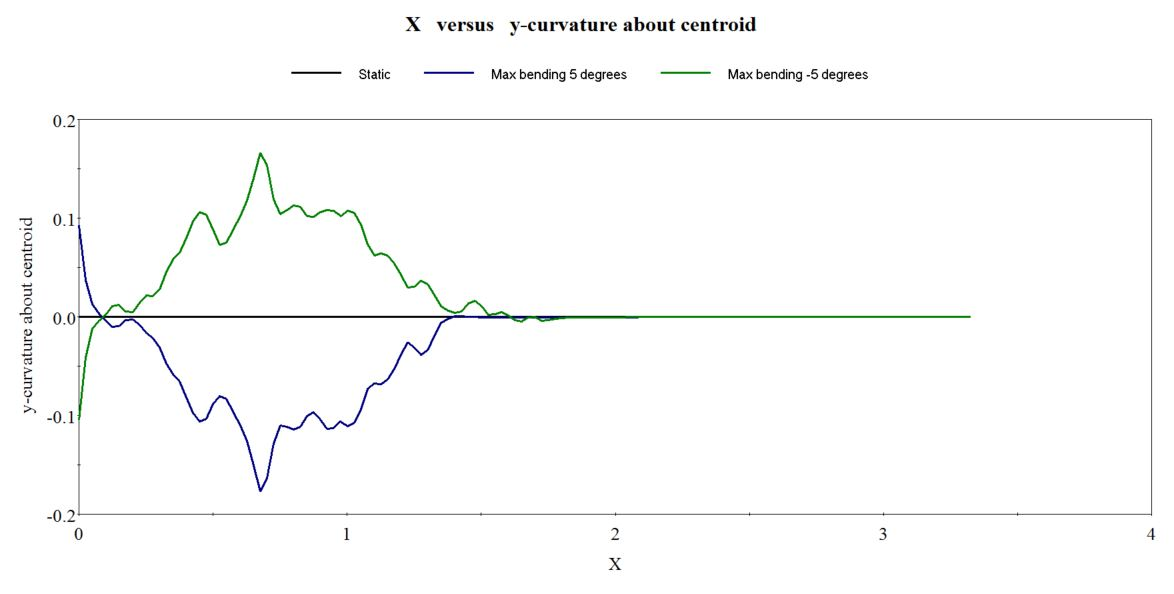
\includegraphics[scale=0.75]{figures/bflexcurve}
\caption[$\; \:$Curvature in outer sheath]{Curvature in the outer sheath over the length of cable}
 \label{fig:bflexmz}
\end{figure}
\noindent Figure \ref{fig:bflexmx} presents the curvature over the length of cable. The curvature plot does not have the desired shape, and there is curvature at x=0. This indicates that the bend stiffener is not doing its purpose, and that it might be too short. This definitely has to be looked at in the master thesis. \newline
\newline
The local model has been assessed in the figure above. As mentioned, it seems that the bend stiffener is not performing in a satisfactory manner, and this will need to be investigated further. As with the global model, the local model is somewhat simplified and based on assumptions Creating the model has given the author a greater understanding of local models and of the software BFLEX, and is considered to be at least a starting point for the local analyses that will take place in the master thesis.   